\section {文件与文档概述}

.
    \begin{center}
        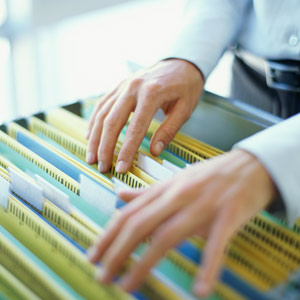
\includegraphics[scale=0.7] {pickfile.jpg}
    \end{center}

    \subsection {文件管理的定义}

    1982 年 6 月,联合国教科文组织与国际档案理事会在联邦德国柏林的普鲁士文化遗产国家图书馆共同主持召开了“文件与档案管理规划第二次专家协商会议”。这次会议把“文件管理”解释为:“文件管理是指对文件在其形成、保存、利用和处置过程中进行的经济而有效的全面管理。文件管理概念的内涵包括文件生命周期中从文件的形成或接收到它们的处置过程。”这代表了目前国际档案界对文件管理及其含义的认识。美国是最早开始研究文件管理的国家之一,1976 年美国颁布了《美利坚合众国联邦文件管理法》,该法在 2 901 条中为文件管理下的定义是指“与涉及文件产生、保管、利用、处置等有关的计划、管理、指导、组织、训练、发展等的管理活动”。在这之后,美国国家档案与文件署对这一定义做出了比较详细的解释:“文件管理包括对文件从产生到最后销毁,或为永久保存而移交到档案馆的生命过程的控制活动。它包括保证文件的有效利用,防止工作中产生和使用一些不重要的便条式的文件,改善文件的整理和收集方式,在文件中心为文件提供专门的管理和廉价的存储,确保日常工作中使用时不再对文件进行专门处理。”

    英国现代档案学者迈克尔· 库克在 20 世纪 70 年代主要从范围和职能上对文件管理进行了深入研究。他认为文件管理的主要职能是控制文件转化为档案的过程。其实质性工作是收集、处理和保管过时文件,并从中鉴定具有潜在价值的文件,作为档案永久保存。

    由此可见,各国关于文件管理含义的表述具有三个共同点:第一,文件管理的基础是文件生命周期理论。根据文件生命阶段的不同特点,采取最为适宜的管理方法,满足利用需求。第二,以文件生命周期的阶段性为基础的,都强调对文件按其生命过程的阶段性进行有效控制。第三,文件管理都是以经济、有效为目标。

    \subsection {文件管理与档案管理}

    文件管理与档案管理是文件运动过程中的不同管理阶段,各自具有独立的工作对象、工作内容、管理原则和方法,但由于二者的“血缘”联系,又决定了二者之间存在无法割断的关联。首先,文件管理是档案管理的前提。档案是由文件转化而来,那么文件的质量将直接决定档案的质量,文件管理的好坏也将直接决定档案管理的优劣。

    文件转化为档案,并不意味着文件管理的终结,而是作为文件管理的继续和发展形势,仍然发挥着重要作用。因此,文件管理和档案管理既是两个独立的管理系统,同时又是更大的文件运动系统的子系统。在管理中,应高屋建瓴地对其统筹规划,使之彼此关照,共同完成系统目标。

    电子文件与文档与传统意义上的档案既有联系又有区别。其主要的联系是,电子文件与文档中的一部分内容是由传统意义上的档案经过数字化转化而来的。

    其主要的区别在于:电子文档是全数字化形式存在的信息,而传统意义上档案则基本上以传统物理形式存在;电子文档比传统档案的范围更广泛,电子文档不仅包含档案类文件,而且包括大量非档案类文件,如临时文件、工作文件等;档案只是已经结束流转过程,进入归档状态的静态文档,电子文档既包括静态文档,又包括处于流转过程中的动态文档;其设计思想存在根本的差异,档案管理系统的基本设计思想是将档案管住,因此基本上是一个封闭的系统,在开放性方面存在严重不足,而电子文档管理系统的基本设计思想是将信息资料用起来,其重心在“用”字上,因此基本上是一个开放的系统,具有充分的开放性,能有效满足网络经济时代对信息的需求。

    \subsubsection {文件管理的特征}

    对企事业单位来说,文件管理虽然不是组织的各项职能本身,但组织管理中的计划、决策、组织、指挥、控制、协调等职能的实现无不依赖高质量、高效率的文件管理。离开了文件和有效的文件管理工作,就难以有效地行使管理职能。而文件管理在现实管理活动中的这种重要地位和不可替代的作用都是由其自身具有的独特性质决定的,具体表现如下。

    \begin{enumerate.zh}
        \item 服务性。从本质上说,管理即服务。文书文件管理应为企业实现自身职能提供高效优质的信息服务。文件管理不是组织管理的目的,而是为了达到管理目标而采用的手段,通过文件管理信息系统为企业和其他社会组织的科学、正确决策提供文件信息支持,其工作的目的是最大限度地满足其职能部门的文件信息需求。这种服务通过接收、加工信息等辅助性工作表现出来,将企业制发的决策信息以有效快捷的方式传递出去,再将相应的信息反馈回来,为检验、修正、完善各类组织的决策提供信息保证。它与企业管理活动同步进行,并成为企业工作不可缺少的参谋和助手。

        \item 技术性。文件作为信息传递的一种工具,其形成、传递、处理、存储等管理活动都具有相对独立的方法、手段和规则,都具有鲜明的技术特征。此外,现代科学技术运用于文件管理活动使其技术性得到进一步的提升,特别是计算机与网络的运用。不掌握这些技术,就无法实现现代文件管理。

        \item 时效性。文件在特定的时间和空间范围内对特定的组织或人员具有指挥、命令、批准、允许、交换和传递信息等执行效用,而要使这种效用得以充分发挥就要求文件管理工作必须做到及时迅速,讲求实效。如果文件办理过程拖沓推诿,必然延长甚至延迟文件的办理,事过境迁,文件便难以发挥应有的效用。这样,文件管理工作不但在组织管理活动中起不到助手的作用,反而会误时误事,降低工作效率,造成工作损失。因此,在文件管理工作中应当科学地安排时间,合理压缩文件的运转周期,降低非实质性办理环节的时间耗费,提高运行速度,尽量消除无效停滞时间消耗,将有效停滞时间消耗降低在必要限度内,充分发掘时间的利用价值,努力维护其时效,使文件得到及时、适时的处理。保证文件能在其有效的时间范围内,最大限度地发挥功能,产生效用,推动各项管理活动的开展。
    \end{enumerate.zh}

    \subsection {文件管理的理论依据}

    实施文件管理的主要理论依据是系统论、文件生命周期与文件连续体理论。

    “系统”一词来自拉丁语,是“群”与“集合”的意思。在韦氏大辞典中,“系统”一词定义为“有组织的或被组织化的整体”,是“形成集合整体的各种概念、原理的综合”,是“以有规律的相互作用或相互依存形式结合起来的对象的集合”。因此,“系统”可以定义为具有一定功能的、相互间具有有机联系的、由许多要素组成的整体。这些组成部分通常被称为子系统,而这个系统本身又可以看作为它所属的那个更大系统的组成部分,在这个意义上,系统与子系统之间具有相对性。系统具有整体性,系统内部各要素之间具有有机联系性,而且这种联系性表现出多层次、多结构,这些层次与结构之间的分布会随着时间的变化而变化,并与系统外部发生着物质、能量、信息的动态交换,从而使系统本身的有序性发生变换。

    依据系统思想建立起来的完整科学体系称为系统科学。它的基础理论是系统学;它的技术基础是运筹学、控制论、信息论等;它的应用技术是系统工程。系统工程是处理系统的工程技术,其目的是使系统达到整体最优或满意。

    系统理论要求在文件管理工作过程中,将文件管理工作视为一个有机的系统或整个企业中的一个子系统。它必须要与整个组织的所有工作形成一个有机整体或一个大的系统。没有文件、信息,没有畅通的文件、信息渠道,没有良好的文件和信息的管理,组织就会指挥不灵,系统就可能崩溃。因此,建立文件信息管理系统来科学地组织和控制文件信息流,是任何组织实现管理目标的重要环节。

    文件生命周期理论和文件连续体理论揭示了文件运动的基本规律。它们的贡献在于根据文件的不同价值将文件运动过程划分为不同的阶段,在每一个阶段上根据文件的具体情况制定不同的管理原则,采取不同的管理方法。文件从产生到最终销毁或转化为档案永久保存,经历了一个连续而又具有不同特征的运动过程。根据各个阶段文件信息运动变化的特点,设计出与之相适应的管理程序,达到以最经济和最有效率的方式组织、控制、保管文件信息,最大限度地满足人们有效利用的目的。

    \subsubsection {文件管理的原则}

    文件管理在各项管理活动中发挥着特殊的效用,文件管理的好坏直接影响企业各项管理活动的质量和效率。为了提供高质量的服务,文件管理必须遵循集中、法制、精简、高效的原则,并建立一系列的管理制度,以确保文件管理的高质量、高效率。文件管理的基本原则如下。

    \begin{enumerate.zh}
        \item 集中原则。集中原则,即对文件管理实行集中统一的领导、指导,建立高度统一的制度、规范,对部分文件实行集中处理。

        企业领导人应负责对本企业文件管理活动的领导,日常文件工作活动的组织、协调工作由其授权的综合办公部门具体负责。上级机关的综合办公部门有权对本系统的下级机关的文件管理活动实施业务指导和监督,并有权根据本系统、本企业的实际情况,制定统一的文件管理办法、制度、规范标准,以消除企业之间、部门之间、工作人员之间在理解、贯彻、组织实施中的障碍,保证各级各类组织的文件规范化和标准化。

        集中原则还表现在文件办理环节的集中统一,即文件管理中的一些具体工作,如签收、登记、分发、组织传阅、信息加工、归卷、催办、查办、立卷归档等各项具体管理工作。在一个具体组织中,一般均由文书处理部门的专职或兼职文件工作人员负责处理,集中统一组织收文、发文以及文件的传阅运转工作。

        集中原则特别强调在文件管理领导体制上的集中,而在具体的文件处理和处置中并不是要求绝对的集中,并不意味着一个组织的全部文件都要集中到综合部门或某一个部门来处理,仍然允许出现分层分工管理文件,这取决于一个组织的内部机构的架构、层次深度以及文件的数量等多种因素。

        \item 法制原则。法制原则,是指依照国家有关法律、法规、规章制度等对文件工作各要素及文件处理活动进行组织、协调、规范,依法制发、传递、处理、存储文件。

        根据法制原则,必须要制定并严格实施各类法规、规范和制度,建立文件管理工作的秩序和工作行为准则,为高质量高效率的文件工作提供依据和保障。

        文件管理工作人员在其文件管理过程中必须依法办事,严格执行法律法规和标准、规范的内容。由于企业管理活动的过程从一定意义上就是文件管理的过程,因此文件管理必须强调程序,必须依法、依程序办事。否则,将造成管理混乱,严重危害依法行政、依法管理的各项活动的正常运行。

        \item 精简原则。精简原则,即在文件管理中将文件与文件管理工作中具有重复性、相关性以及多样性的各要素、各环节化繁为简,去粗取精,以实现文件管理系统的整体最优功效。

        首先,简化机构,根据组织的规模、层次的多少和职能活动内容以及文件数量等各种要素合理设置文件管理机构,并配备高素质的文件管理人员,明确岗位职责。

        其次,对文件管理的过程尽可能简化,这包括简化工作过程,简化操作程序,简化手续。另外,对文件本身也需要简化。例如简化文件的结构、文件的字数、文件的种类等。

        \item 效能原则。效能原则,即是在实现文件管理目标的前提下考虑以最少的人力、物力、财力和时间的投入,经济高效地完成文件管理各项工作。

        文件管理应树立成本控制的观念。根据投入产出原则评价管理工作。根据国家的有关规定和文件与文档管理工作的特点,应建立以下制度。
            \begin{enumerate}
                \item  写作制度。这是指文件写作中应遵循的原则、规则和程序,包括规定文件体式、结构和格式,文件语言运用,文件内容要求,文件撰写程序与方法,文件主题词撰写方法,规定文件种类的划分原则,文种的表示方法、用途,选择文种的依据等。
                \item  审核签发制度。具体包括规范文稿审核的范围、审核程序、审核内容,审核人的责任及任职资格条件,审核修改文稿方式,要禁止出现多头主送,滥抄滥报,违制越级行文现象;文件签发权限,签发人责任,签发程序,签发的种类,会商会签的范围形式和程序手段等,注意正签、代签、核签、会签的区别,不得越权签发文件,要强调文件应“先核后签”等。
                \item  缮印制度。具体包括规定缮印范围、批准手续,缮印方式及其选择依据;缮印前定稿的规范化处理,版式设计规范,校对的方式、次数与责任者;纸张和各种字迹材料的材质选择,规格要求,缮印时的期限与缮印数量等。
                \item  用印制度。具体包括印章的使用范围,批准使用程序,印模使用规则,监印方法要求,印章管理者的责任与任职资格规定等。
                \item  保密制度。这是指在文件管理活动中应严格执行有关保密工作的法律、法规和规章,严守党和国家的秘密以及其他组织管理中的工作秘密,以确保文件的安全。
            \end{enumerate}
    \end{enumerate.zh}

\subsection {文档管理的基本内容}

    传统的手工文档管理形成了许多文档组织和交换的方法,这些方法在实践中被证明是行之有效的,电子文档管理也需要反映和利用这些方法。以下通过手工文档管理和电子文档管理的对照来讨论文档管理的基本操作。

    \begin{enumerate}
    \item 文档的建立
        \begin{itemize}
            \item  手工文档。在建立文档之前要进行文档规划,例如列出初步的文档清单、制定文档的标准格式等。一旦文档被建立,文档的页眉、标题等就根据文档的内容通过标准化的方式填写。
            \item  电子文档。在计算机处理方式下,文档规划是通过在文档数据库中进行注册来完成。文档规划时,在数据库中定义文档进入系统时所需要的信息项,如关键字、标题等。在文档被创建时,系统根据预先定义好的信息项,要求作者填写相关内容。
        \end{itemize}

    \item 文档的分发
        \begin{itemize}
            \item  手工文档。文档是根据既定的发送清单来分发的,并提供包含了文档状态和有关发送细节信息的信函,接收方在收到文档时进行确认。
            \item  电子文档。使用计算机网络通过数据传送功能完成文档的分发,计算机可以根据电子格式的发送清单中定义的发送目标自动地进行发送。也可不进行实际的文档发送,而是将文档储存在项目成员者能使用的文件服务器中,加入新文档或更新版本时对发送清单中的所有人员发送通知,再由收件人访问文件服务器查阅文档。在这种情况下可以通过使用适当的监控方式如文档日志等,记录所有的有关文档存储、通知发送、接收和阅读的信息。
        \end{itemize}

    \item 文档的检查和批准
        \begin{itemize}
            \item  手工文档。在文档能用于最终目的时,通常要经过一定的审批程序。典型的工作流程首先是文档发送方内部对文档进行校对,然后由其他专家和领导进行审阅,在进行必要的调整后作出最终的批准,并签字盖章。随后每一次对文档进行的修改,原则上都要采用相同的检查与审批程序。
            \item  电子文档。工作流程应用程序的使用可以使批准过程自动化,并使用电子签名和电子印章确认批准,这既可以用于一个项目,也可以仅用于某一文档或文档类别。
        \end{itemize}

    \item 文档的储存和检索利用
        \begin{itemize}
            \item  手工文档。文档被按一定的顺序储存起来以方便查找和改正。文档通常放在文件夹、装订机和抽屉里,在一个企业内部一般是采用标准的方式储存。
            \item  电子文档。几乎所有的计算机系统在初级层次上都采用文件目录结构对文档进行组织,这类似于手工方法里的文件柜。对文档的检索和修改是电子文档管理系统的基本功能。检索建立在元数据或文档内容的基础上。对于图形文档,因为图形格式识别技术还未成熟,元数据是最常用的检索技术;同时,尽管许多文本文档通过全文检索就能被成功地查找,但如果加上关键词或其他元数据就能大大提高检索的质量。
        \end{itemize}

    \item 文档的存档和删除
        \begin{itemize}
            \item  手工文档。某项任务或工程完成后,文档有的可以被直接销毁,有的需长期保存,以便用于其他项目。需要保存的文档就必须存档,通常的手工方法是统一装订有用的项目文档并对文档进行索引,以方便以后的文档查找工作。并且通过存档,人们对在项目建设和维修期间的文档进行的储存和分类有利于文档管理。
            \item  电子文档。不再需要的文档可以删除,有保留价值的则可统一存储在可靠的存储介质上,被妥善保管。通过使用文件结构和元数据,计算机文档检索可以更快、更有效地完成。改变数据格式和储存媒介时,要注意保持文档的长期可读性。
        \end{itemize}
    \end{enumerate}

\section {电子文档管理}

\subsection {电子文件与文档管理的价值}

    认真实施电子文件与文档管理,除了会明显提升企业和组织的形象,提高办事效率外,还将对组织的作用和价值得到极大的提升。这表现在以下几方面。

    \begin{enumerate}
        \item 促进信息交流。通过电子文档管理系统的应用,更加方便组织里的人或人群之间的交流,电子文档管理系统支持跨越时间和空间的信息传送。上情下达和下情上传将更加畅通。

        \item 提高组织利用知识的能力。文档形成了组织“记忆”的重要组成部分,大量的知识保存在电子文档中,文档管理系统通过数据挖掘,提供文档的结构、内容方面的更加清晰的查询与共享,使组织能够分析文档内容的相互关系,使存储在文档中的知识更加系统化,从而提高组织整体上利用知识的能力。
    \end{enumerate}

    电子文件与文档管理的原则电子文件与文档管理的目标主要是保障电子文件的真实性、完整性和长期可读性。

    真实性是保证电子文件行政有效性和法律证据性的基础,是电子文件反映历史面貌,构成社会价值,得以作为社会记忆长久保存的前提。

    电子文件的完整性包括三个方面的含义,一是作为记录社会活动真实面貌的具有有机联系的电子文件及其他形式的相关文件数量齐全;二是每一份电子文件的内容、结构和背景信息没有缺损;三是与主文件相关的支持性、辅助性、工具性文件齐全。

    电子文件的可读性是指文件经过存储、传输、压缩、加密、媒体转换、迁移等处理后能够以让人可以识读、可以理解的方式输出。电子文件的可读性是其具有存在和保存价值的基础,如果文件不能顺利读出,文件中的信息便成为“死信息”。

    为此,电子文件与文档有如下的管理原则。

    \begin{enumerate}
        \item 全程管理原则。电子文件从其形成到销毁或永久保存整个生命周期,应建立一个完整的管理体制,并做到全面的管理,系统的管理,过程的管理。
            \begin{itemize}
                \item  全面的管理。从文件的生成流程、管理规则、管理方法及质量要求出发,需要建立一个涵盖电子文件全部管理活动的目标管理体系、程序体系和技术方法体系。
                \item  系统的管理。要注重电子文件生命周期内各个阶段所有管理活动和管理要素的统筹兼顾,强调各项管理内容和要求的无缝链接。注重充分利用管理系统的各种资源,以知识管理的理念,追求系统资源和信息资源最大共享和最大效益。
                \item  过程的管理。通过过程控制实现结果的控制。对每个过程监控以达到对最后结果的控制,使系统每个过程产生的信息自动记录在案。以保证电子文件在其整个生命周期受到严密的控制,体现全程管理的思想。以保证文件的行政有效性和法律有效性。
            \end{itemize}

        全程管理的框架模式——管理链,这可描述为:根据预先确定的标准格式和模板编辑文件→根据文件的类型和用途使用预先确定的方法认证文件→根据人的资格及其权限确定他接触电子文件的权力→在系统中嵌入工作流程并只向有关人员呈现有关的文件→使用磁卡、密码、指纹识别等方式限制某些人员的接触→在系统内设计跟踪功能。

        \item 前端控制原则。前端控制是现代文件和档案管理理念的重要内容,以文件生命周期理论为基础,把文件从形成到永久保存或销毁的不同阶段看成一个完整的过程。文件形成为前端,处理、鉴定、整理、编目等具体管理活动是中端,销毁或永久保存为末端。要对文件形成前端的有效管理,电子文件的管理必须延伸到系统设计端,把各项管理过程的目标、要求和规则进行系统分析、科学整合并纳入到系统功能之中,只有实施前端控制,才能实现全程管理。

        前端控制是电子文件真实可靠、完整安全、长期可读的有效策略。根据电子文件的易流失、易修改等特性,在系统中增加措施,贯穿于文件的形成过程,可以有效地防止其他管理环节对电子文件的损伤和破坏。例如:归档范围加到电子文件管理系统之中,属于该范围的文件一“出生”,就被加上归档标识,使之具有防止修改、防止删除的属性,并生成相应的描述信息,从而确保电子文件安全留存和内容真实性。

        电子文件管理系统不是手工管理流程的简单模拟,即需要“业务流程的重构”。要尽可能地减少和消除文件、档案管理全程中各个管理环节的重复、疏漏和冲突,从而达到功能合理,效率最高。

        \item 真实性保障原则。电子文件的真实性是指文件的内容、结构、背景信息经过传输、迁移等处理后依然保持不变,与形成时的原始状态一致。随技术环境迁移,维持法律凭证的作用,但维护电子文件的真实性是很困难的。电子文件的法律凭证效力是基于其信息内容的原始性,为维护电子文件的原始性,目前我国在《电子文件归档与管理规范》(GB/T 18894—2002)规定了 4 条措施:
            \begin{enumerate}
                \item  建立对电子文件的操作者可靠的身份识别与权限控制;
                \item  设置符合安全要求的操作日志记录,随时自动记录实施操作的人员、时间、设备、项目、内容等;
                \item  对电子文件采用防错漏和防调换的标记;
                \item  对电子化的印章、数字签名等采取防止非法使用的措施。
            \end{enumerate}

        国际电子文件真实性的永久保管在国际研究项目中也规定了 4 项措施:确认不同类型电子文件的要素对真实性产生的影响,以便对要素加以记录和保护;对电子文件不可视的部分变成可显示的,并通过文件的智能链接,使可视性得到固定;以上两条失败后,把文件转制为非数字式文件,内容可记录下来;对文件的迁移采用自我记录和自我认定的办法以及不间断的物理管理。

        总之,真实性保障解决方案主要是采用事前控制、事中跟踪记录和事后审查等措施;基于政策、方针、程序、制度、标准的管理框架和基于系统软件硬件环境、加密、签署、认证的技术框架等,从不同角度对电子文件的真实性认证和维护进行保障。

        \item 完整性保障原则。电子文件的完整性是指电子文件的内容、背景、元数据等信息无缺损。它包括两个方面的含义,一是作为记录社会活动真实面貌的具有有机联系的电子文件及其他形式的相关文件与文档保存完整齐全,保证相互印证;二是电子文件的内容、结构和背景信息没有缺损。完整性是电子文件价值的重要保障,残缺不全的文件留给后人的是残缺不全的社会记忆,以致不能作为凭证采用。

        \item 有效性保障原则。电子文件的有效性是指文件经过存储、传输、迁移、加密、压缩、媒体转换以及软硬件环境变动后,仍能够以人们可理解、可被利用的方式输出,并保持其内容的真实性。包括信息的可识别性、存储系统的可靠性、载体的完好性和兼容性。有效性措施贯穿于电子文件的全程管理中。归档时应根据电子文件的类型和特点注明文件存储格式、软硬件环境、相关的数据信息参数等。对电子文件的鉴定要从内容和技术状态两个方面进行分析,有效性检测是技术分析的内容之一。在实际工作中应建立电子文件有效性管理制度并采取相应的技术保证措施。

        在《电子文件归档与管理规范》(GB/T l8894—2002)中对电子文件有效性规定了 4 条措施,这些措施是:
            \begin{enumerate}
                \item  归档电子文件的形成单位和档案保管部门每年均应对电子文件的读取、处理设备的更新情况进行一次检查登记。设备环境更新时应确认库存载体与新设备的兼容性;如不兼容,应进行归档电子文件的载体转换工作,原载体保留时间不少于 3 年。保留期满后对可擦写载体清除后重复使用,不可清除内容的载体应按保密要求进行处置。
                \item  对磁性载体每满 2 年、光盘每满 4 年进行一次抽样机读检验,抽样率不低于 10%,如发现问题应及时采取恢复措施。
                \item  对磁性载体上的电子文件,应每 4 年转存一次。原载体同时保留时间不少于 4 年。
                \item  档案保管部门应定期将检验结果填入《归档电子文件管理登记表》。
            \end{enumerate}

        电子文件的真实性、完整性和有效性保证,应建立规范的制度和工作程序并结合相应的技术措施,从电子文件形成开始不间断地对有关处理操作进行管理登记,保证电子文件的产生、处理过程符合规范。电子文件的处理和保存应符合国家的安全保密规定,针对自然灾害、非法操作、病毒侵害等采取与系统安全和保密等级要求相符的防范对策,例如:网络设备安全保证,数据安全保证,操作安全保证,身份识别方法等。

        \item 可靠性原则。电子文件与文档的可靠性是关系到电子文件凭证效用的关键因素,它涉及电子文件管理中的每一个环节。总的说来,需要从技术、管理和法律三个方面入手,共同确保电子文件的可靠性及其法律效力。

        电子文件是高科技的产物,它的各种性能是由技术决定的。随着电子文件的广泛使用,信息安全技术就显得特别重要,电子文件的制作者、管理者都应积极采用有关技术措施,提高电子文件的可靠性。目前,用于维护电子文件真实性、安全性方面的技术,主要有加密技术、签署技术、消息认证、身份验证、防火墙等技术手段。

        和纸质文件相比,电子文件的管理不仅注重每个阶段的结果,也重视每一项工作的具体过程,并把这些过程一一记录下来。具体包括对参加电子文件制作和管理的人员进行审查,从源头上保证电子文件的可靠性;建立电子文件全过程管理制度,明确各方面的职责要求,为每一份电子文件建立必要的记录,从收集、积累开始就要进行记录,记录电子文件的管理和使用情况,等等。

        \item 可读性原则。影响电子文件可读性的因素很多,如软硬件的过时、加密、载体的损坏等,都会造成记忆的丧失。这些对于长久保存的电子文件来说,是极为不利的。

        离开电子计算机软硬件平台,电子文件既看不见也摸不着。由于电子文件对设备依赖性和对其他设备环境的不兼容性,使其只能通过特定的机器来识读,有时还只能在某种特定的设备上处理;不同软件环境形成的电子文件存储在载体上,有时难以互换;电子文件加密后,不解密就无法识别;技术设备更新时,如不及时解决格式转换问题,也就无法读取。因此在管理电子文件时必须利用各种手段保存各种背景数据,保证电子文件在不同时空范围内可以顺利读取文件信息,否则,就失去了管理电子文件的目的和意义。

        \item 集成管理原则。集成管理是对管理要素的科学重组,是全程管理思想的延伸和深化。包括文件流内部管理活动的集成、文件流与业务流的集成、文件流与其他信息流的集成等。在信息技术和网络技术飞速发展的形势下,电子文件与文档管理必将向分布式、网格化、知识化方向发展。届时,信息的集成和整合更是势在必行的了。
    \end{enumerate}

    \subsection {电子文档管理的功能需求}

    与纸质文件管理一样,电子文件的管理同样要经过鉴定筛选,将反映本企业职能活动的具有保存价值的文档信息保存下来,并为组织及其内部机构开展业务活动提供方便快捷的电子信息服务。但二者在管理原则、程序、方法与措施等方面都存在着很大的差异。下面将分别予以介绍。

    \subsubsection {电子文档的收集}

    随着我国社会信息化进程的快速推进,电子政务和电子商务日益成熟和发展,电子文件产生的领域不断拓展,产生的文件数量急剧增长。但是,目前存在许多问题,例如:草稿性电子文件存在“自生自灭”的情况;辅助性电子文件处于无人管理的状态;正式电子文件往往只进行了逻辑归档,也就是说电子文件生成时保存在什么位置,归档后仍不改变,电子文件容易丢失;有些电子文件的存储载体不安全,信息记录格式不标准。为了有效地避免以上问题,根据前端控制的原则,针对电子文件产生状态的分散性,必须从办公自动化等系统设计开始就采取措施,从技术上保证电子文件收集工作的有效性。电子文件收集除了要在文件归档时进行常规收集外,还要弄清楚电子文件产生的渠道,积极主动地做好电子文件的全面管理工作。为此,必须规定电子文件的收集范围。由于电子文件的快速流动性、变换性等特性,要特别注意即时和实时收集和积累电子文件。

    电子文件的收集范围应该包括两大类:前台文件和后台文件。前台文件是反映本部门职能的各类电子文件,是归档电子文件的主体,它反映文件的内容,是捕获的主要对象。这类文件捕获时应注意既应该保存定稿也应注意保存草稿,使归档的数据能反映各类文件在起草、修改、审核直至签发的每一个环节中责任人的意志,以保证历史的真实性。后台文件包括操作系统、语言处理系统与用户应用程序等。

    根据《电子文件归档与电子档案管理规范》规定,对电子文件的捕获主要有以下几方面的要求。

    \begin{enumerate}
        \item 记录了重要文件的主要修改过程,有查考价值的电子文件应保留。当正式文件是纸质材料时,如果保管部门已实施计算机处理,则与正式文件定稿内容相同的草稿性电子文件应当保留,否则可根据实际条件和需要,确定是否可以保留。
        \item 保存与纸质等文件内容相同的电子文件时,要与纸质等文件之间建立准确、可靠的标识关系。
        \item 在“无纸化”办公和事务系统中产生的电子文件,应采取更严格的安全措施,保证电子文件不被非正常改动。同时必须随时备份,存储于能够脱机保存的载体上,并对有档案价值的电子文件制作纸质或缩微胶片拷贝件保留。
        \item 用特定文字处理技术形成的电子文件,捕获时应注意文件的存储格式和属性。
        \item 用扫描仪等设备获得的图形电子文件,如果采用非标准压缩算法,则应将相关软件一并收集。
        \item 用计算机辅助设计和绘图等获得的图形电子文件,收集时应注意其对设备的依赖性,以及易修改性等问题,不可遗漏相关软件和各种数据。
        \item 用视频设备(视频捕捉卡等)获得的动态图像文件,收集时应注意收集其压缩算法和软件。
        \item 用音频设备获得的文件,收集时应注意收集其属性标识和相关软件。由计算机多媒体技术制作的文件,收集时应注意收集其压缩算法和属性标识及其软件。收集时应注意参数准确、数据完整。
        \item 通用软件产生的电子文件,收集时应注意收集其软件型号和相关参数。专用软件产生的电子文件,收集时必须连同专用软件一并收集。
        \item 计算机系统运行和信息处理等过程中涉及的各类参数、管理数据等应与电子文件一同收集。
    \end{enumerate}

    为了维护电子文件的完整性,电子文件的捕获除按照以上的要求进行之外,还需注意以下问题:文件内容必须能准确反映在特定时间内,在行使职权和履行职责的活动与事务处理中的全部过程。

    对捕获到的电子文件应及时按照要求制作电子文件备份,并填写《电子文件登记表》,电子文件登记表如果制作成电子表格,应与电子文件一同保存,并附有纸张打印件。

    \subsubsection {电子文件的鉴定}

    电子文件鉴定工作的内容具体包括鉴别、内容与技术状况的鉴定、处置、记录等环节。鉴别工作就是确定哪些信息是文件,从而判断其价值。鉴别是电子文件鉴定工作的第一步,也是鉴定工作顺利开展的基础和前提。鉴别的任务是将文件从非文件信息中挑选出来,其实质是明确机构形成电子文件的需求,即机构需要形成哪些电子文件。

    \begin{itemize}
    \item 电子文件的技术鉴定。电子文件的技术鉴定可以分为三个方面,即:对电子文件物质载体状况的鉴定,这包括介质物理性能的鉴定和对介质媒体形式、存储格式的鉴定,亦即文件信息真实性鉴定;对电子文件的完整性、可读性的鉴定;对电子文件有无病毒的鉴定。在以上多方面物理鉴定和文件信息价值鉴定的基础之上,进行保管费用和价值的权衡。
        \begin{enumerate}
            \item  真实性鉴定。鉴定电子文件的真实性,主要是认定文件是否就是当时、当人、当事形成的,也就是说,可以将真实性理解为“原始性”。就电子文件软硬件依赖性所造成的真实性问题,可采取以下措施。第一,分析机构内各类电子文件中哪些组成要素能确保文件长期的真实性;第二,根据预先确定的标准格式和模板编辑文件;第三,对于某些文件可将该文件转换成非数字形式,如缩微等;第四,对文件的迁移进行记录。
            \item  完整性鉴定。这分为检查文件要素和检查要素集中手段两个方面。前者是指利用有效的技术手段,对照元数据模型,检查文件各个要素是否完备,包括可视和不可视的部分。后者是指分析联系文件各个要素的手段是否有效,这些手段包括超级链接、置标语言等。
            \item  可读性鉴定。可读性鉴定是电子文件技术鉴定的重要内容,目的在于确认电子文件中的内容可以正常读出,没有丢失和差错。这不仅需要确认文件在形成时的可读状态,同时需要分析其是否具备日后多次无差错读出的技术性能。主要包括检查与电子文件相配套的软件、相关的电子文档、文字材料是否齐全、完整,对于加密文件的密码是否保存;检查电子文件的信息存储格式是否符合归档要求;核实归档或迁移时填写的文件运行的软硬件环境、版本号是否正确;检测在指定的环境平台上能否准确读出电子文件并确定其是否值得保存等工作。
            \item  有无病毒鉴定。可运用病毒检测软件检测归档文件和归档介质是否携带病毒。
            \item  介质状况检测。检测介质物理性能,如检测磁带或光盘是否清洁,介质表面是否光滑、无皱褶、无划伤、无磨损,运转是否正常等;检查介质规格是否标准。
        \end{enumerate}

    \item 电子文件内容鉴定方法。内容鉴定是电子文件鉴定的主要内容,其中主要的鉴定方法理论有:职能鉴定法、内容鉴定法、直接鉴定法、行政官员鉴定论、利用决定论等。这些方法是从不同角度不同侧面进行鉴定,其目标都是力求鉴定结果的客观、准确。其中职能鉴定法和内容鉴定法是电子文件鉴定的两种基本方法。
        \begin{enumerate}
            \item  职能鉴定法。

            职能鉴定法是指按照立档单位在企业中的地位和职能的重要性来确定文件的价值。社会组织的运转通过各机构职能的履行而实现,文件是职能活动的真实记录,因此,文件价值的大小取决于职能活动的重要程度,以职能因素为标准鉴定文件能较为客观地反映各个历史时期社会的真实状态。采用职能鉴定法鉴定电子文件,效率较高。职能鉴定法依据机构各种事务活动的重要程度,分别予以处置。因此,职能鉴定法具有从总体上判断机构形成文件的价值的能力,而不是直接对文件加以处理,表现为“批处理”的方式,反而对于电子文件的鉴定更有效率。
            \item  内容鉴定法。

            计算机是电子文件内容鉴定的最终执行者,是保存和销毁电子文件的实际场所。最理想的内容鉴定应由计算机自动进行,这必须建立在计算机智能化程度很高的基础上,因此难度很大。在不能开展自动鉴定工作的机构,则由人工执行。有些单位采取自动鉴定和人工鉴定相结合的方式。
        \end{enumerate}
    \end{itemize}

    \subsubsection {电子文件的整理}

    没有整理的电子文件只能是杂乱无章的电子信息,重要文件信息就难以搜索到,也就无法有效地利用文件。因此,电子文件的整理是实现电子文件管理目标的重要条件。

    电子文件的整理,是指按照一定原则和方法,将电子文件分门别类系统化、有序化的一项工作。电子文件的整理工作包括分类、排序和建立数据库两个层次。

    \begin{enumerate.zh}
        \item 分类、排序。分类、排序是将收集到的零散和杂乱的电子文件通过分类、标引、组合,使电子文件存储处于有序状态。由于存在不同系统产生的电子文件,在整理过程中,可能会遇到文件格式重新编排和组合的问题。这种格式转换有可能损伤数据,损害电子文件的凭证作用。电子文件分类排序、著录标引是保管电子文件的基本要求,在建库前的整理工作中占有重要的地位,其整理的质量直接影响电子文件的保管和利用。

        \item 建立数据库。建立数据库前应对电子文件进行分类编号,使其达到总体上的有序。对于不同应用系统应选取不同的文件组织方式或组合方法,目的是方便使用。组建数据库的主要工作内容有:对电子文件进行分类编号,按分类标准,结合专业要求和电子文件内容,制定科学的分类方案。给每份电子文件一个固定的编码,从而使全部电子文件成为一个有机的、排列有序的整体。然后,对电子文件进行登记入库。数据库建立后,要开发检索工具,检索工具是对电子文件进行快速访问的有效手段。
    \end{enumerate.zh}

    有些重要文件还必须以纸质文件管理时,应输出纸质文件一并保存,如法规性的电子文件必须拷贝在纸上保存。对技术、经济、艺术等方面产生的电子文件,保存时间比较短的可按建立数据库整理、存储,不一定非输出纸质文件保存。整理完毕的电子文件应予归档。电子文件归档,是将应归档的电子文件,经过整理确定档案属性后,从电子计算机存储器或其网络存储器上,拷贝刻录到光盘中。

    \subsubsection {电子文件的著录}

    电子文件的著录,是指通过获取、核对、分析、组织和记录关于文件内容、结构、背景以及文件系统的信息,准确描述电子文件的形成过程及其属性。

    电子文件著录具有全要素、全过程、综合性、多级性的特点。

    \begin{enumerate.zh}
        \item 全要素。对于电子文件,需要描述的对象包括文件三要素:内容、结构和背景。因为电子文件具有系统依赖性的特点,因此,文件管理系统也是著录中不可或缺的内容。对文件管理系统的著录不仅包括文件生成时所使用的系统,还应包括文件管理、利用、保存、迁移后所在的各种系统。对于同一份文件的著录可能分散地保存在不同地点,应保证在相同文件的著录之间建立联系。电子文件著录全要素的特点决定了著录的信息源不仅是文件内容本身,还包括生成、管理电子文件的活动过程。
        \item 全过程。著录将贯穿于电子文件的整个生命周期,包括文件编制、处理、归档、迁移、利用等全过程。在这个意义上而言,著录信息是与文件同步形成的,著录时间不再是一个点,而是一个阶段。其中相当多的内容在文件形成时已完成,如文件的生成系统、形成者、编制目的等。著录的全过程与电子文件系统开发的全过程原则是相吻合的。
        \item 综合性。综合性是指著录手段的综合性。电子文件既然是在电子环境下生成的,对于电子文件的著录也应在系统中进行。由于计算机技术和文件、档案工作都是不断趋于成熟与完善的,随着自动化程度的提高,人工直接著录的方式将逐渐演变为系统自动著录和人工控制相结合,其中主要的自动化技术是元数据技术。
        \item 多级性。电子文件著录的多级性是由电子文件之间具有有机联系的特点决定的。根据电子文件之间的有机联系,对文件进行分类,从全宗、大类、属类、小类、案卷直至单份文件,呈现出多个级别、多个层次。针对不同级别的文件集合或文件,著录结果是不同的,但是各级之间的有机联系应始终予以维护。在完善的电子文件检索系统中,应能展现各级著录的层次结构,并提供通畅的导航。
    \end{enumerate.zh}

    结合已有的研究成果,并借鉴《国际档案著录(通则)》制定的电子文件的著录项目。电子文件主要的著录项目有:题名与责任说明项、附件、稿本与文种项、版本及版本说明、密级与保管期限、时间项、载体形态项、附注与提要项、机构史或传记、软硬件平台项、文件类型、编号项、主题词或关键词、检索与利用等。可以看出,以上项目涉及文件内容、结构、背景和文件系统等各个方面的内容。

    \subsubsection {电子文件的归档}

    归档是将电子文件向档案部门移交并存储在存储载体上,以便长期保存的工作过程。《电子公文归档管理暂行办法》第 13 条明确规定:在归档移交前,形成单位应对文件相关项目进行检查,检查项目包括与纸质公文核对内容、签章,审核电子公文收发登记表、操作日志及相关著录条目等,确认电子公文与相关的信息和软件无缺损且未被非正常改动等。确认无误后,方可向档案部门移交归档。不同环境条件产生的电子文件,其归档的方法是不同的,如果是电子计算机网络系统,按要求转到数据库或标记归档的标识,即可完成归档工作。但以存储载体传递的电子文件归档,就必须做一些辅助和认证工作,要与相关的纸质文件结合归档。

    电子文件的归档工作主要包括归档范围、时间、份数、要求、方法等内容。

    \begin{enumerate.zh}
        \item 归档范围。确定电子文件的归档范围,是归档的首要任务,也是保证电子档案质量的关键。一个组织电子文件的归档范围可以参照其纸质文件的归档范围进行归档。与此同时,确定电子文件的归档范围还应遵守以下原则:要根据电子文件的形成规律,尽可能具体列出阶段的、系统的、权威的电子文件组合,保证电子文件的原始性、真实性、完整性;要关注电子计算机的软硬件环境,电子文件内容的基本格式及有关元数据等,应与相应的电子文件、电子文件收发登记表、机读目录、软硬件相关说明等材料一同归档保存。
        \item 归档时间。电子文件一般应在办理完毕后即时归档,也可以在任务完成后,或一个阶段之后进行归档(称为阶段归档) 具体可视其情况而定。,因涉及电子文件的技术环境条件,存储载体的质量、寿命等问题,一般以不超过 2~3 个月为宜。
        \item 归档份数。经分类、整理后的归档电子文件,应拷贝至耐久性好的载体上,一式三套,一套封存保管,一套异地保管,一套提供借阅利用。即使在网上归档,也要拷贝一套封存,必要时应封存两套,其中一套异地保存。因为电子文件在长期保存过程中可能会出现读取错误,但两套都出错的概率就会低很多。另外,存储载体的生产厂商常对存储载体的寿命做出许诺。我们不能以此作为存储载体寿命的依据,因为在存储载体上存放数据时,与出厂时存储载体的技术状态不同、存放的环境条件不同,许多单位达不到厂商提出的保存环境。因此,我们不仅要注意归档的份数,还要注意保存的方法和环境。
        \item 归档要求。对归档电子文件的要求,主要是真实、完整,达到档案的功能价值。首先,要遵从归档各阶段的规定和标准;其次,是准确说明它的软硬件环境。归档保存的电子文件一般不加密,必须加密归档的电子文件应与其解密软件和说明文件一同归档;第三,归档电子文件的格式应为工业标准,在标准的用户界面下操作,支持不同的平台,与现有的设备兼容,能以标准的数据库语言与数据库相连,或者确定统一的标准在内部的电子计算机网络上使用,以实现良好的转换状态;第四,归档电子文件从网上交接的,应注意文件的完整性、安全性及可读性检查;通过脱机存储载体交接的,交接双方均应对其载体和技术环境进行检验,确保载体清洁、无划痕、无病毒等。
        \item 归档方法。无论是电子计算机网络环境,还是微机工作站,其电子文件归档一般采用以下方法:将应归档的电子文件最终版本录入存储载体上,脱机后可存放在别处;对电子计算机网络上应归档的电子文件,经过一段时间积累后进行压缩处理,并录入到存储载体上。这样做对将来的电子档案管理有利;在电子计算机网络环境下采用备份归档,将归档的电子文件在网上进行一次备份操作,录入到存储载体上;“双套制”归档,即同时保存电子文件及其纸质文件形式,一般适用于永久和长期保存的电子文件的归档,这种方法应在两种存储载体中同时保存相应的符合规范要求的机读目录,并在两者之间建立联系,以便检索。
    \end{enumerate.zh}

    电子文件归档经档案部门验收合格后,应填写《电子文件交接检验登记表》 并签字盖章,登记表一式两份,交接双方各存一份。

    \subsubsection {电子文件的保管}

    与纸质文件相比,由于自身的特点不同,电子文件的保管和利用存在自身的特点和要求。

    \begin{enumerate.zh}
    \item 电子文件保管的特点。由于电子文件不同于传统纸质文件,其保管活动也就呈现出如下的特点。
        \begin{enumerate}
            \item  技术难度大。

            电子文件具有软硬件依赖性,在保管电子文件的同时,需要全面考虑再现电子文件涉及的所有因素,只有这样才能够正确地读取和理解文件中的信息。
            \item  成本高。

            电子文件的系统依赖性,增大了电子文件保管成本。电子文件的系统依赖性包括对字符编码、软件、硬件、标准、技术设备更新以及加密技术的依赖。这一特点给电子文件的保管利用带来了巨大的影响,如软件的升级带来的兼容性问题,为保证电子文件长期存取而进行的迁移等。对于电子文件而言,很可能出现存在保存完好的电子文件载体,却无相应的读取环境。要使得电子文件得到有效利用,必须保存完整的读取环境,这无疑会增大管理成本。
            \item  不确定因素多。

            对于电子文件而言,其内容的存储位置是变化的,并不固定依附于特定的载体与特定的位置,它可以通过拷贝的形式附在多个载体上,也能通过分布式存储的方法,将电子文件内容分解后存储于不同的地点和设备,而在需要时才将它们重新组合。这样,同一份电子文件的内容在存储时出现载体分离的现象,在读取这份电子文件时就需要从不同位置的载体中分别进行抽取,如果缺少某一部分内容,则该电子文件的完整性就受到了破坏。另一方面,由于存储介质的可重写性,计算机系统在编辑文件时可以做到不留痕迹地增、删、改。这些不确定因素的存在严重地威胁着电子文件的原始性和真实性,加重了电子文件保管的责任。
            \item  安全系数降低。

            电子文件的共享性在带给用户便利的同时,其信息的安全也面临着威胁。因为电子文件共享性是通过网络环境实现的,但随着网络化的发展,网络安全问题日益凸现,电子文件保管部门应当强化安全意识,采取安全措施,确保电子文件安全。
        \end{enumerate}

    \item 电子文件存储载体的保管。根据以上特点,对电子文件的保管主要包括载体保管、信息保管两个方面。电子文件的载体主要是磁性载体(包括磁带、软磁盘、硬磁盘)和光学载体(光盘),与纸质文件的保管不同,其重点是维护数字记录信号的可读性。具体保护措施如下。
        \begin{enumerate}
            \item  控制适宜的温、湿度。库房温、湿度要相对稳定。

            温度为 15~27℃,变化不得超过±3℃,最佳环境温度是 18℃;相对湿度 40\%~60\%,变化不得超过 5\%,最佳环境相对湿度为 40\%。归档光盘应保存在 14~24℃、相对湿度在 45\%~60\%的环境中。

            \item  防灰尘。

            灰尘可能造成电子文件载体的物理损伤、化学损伤和生物损伤,不仅会使数据丢失,而且还会污染驱动器读写头,甚至传染其他载体。因此,要做好防尘工作,保持环境卫生,减少空气中灰尘的含量,保证装具、机器的清洁。严禁触摸软盘、光盘含有信息的盘体部分,使用完毕要及时放回盘盒中,不应随处存放。

            \item  防止外来电磁场影响。

            外来电磁场特别是强电磁场作用于磁性载体上,能使磁性涂层的剩磁发生变化,造成信号失真,破坏记录信息,影响读出效果。因此,磁性文件载体与电磁场之间要保持安全距离;也可以使用软磁物质(软铁、镍铁合金等)构成载体容器,并通过良好接地,对电磁场进行屏蔽。在存有重要档案的库区应设置测量电磁强度的设备,以查出隐蔽的电磁场。

            \item  防止机械振动。

            机械磨损和强烈振动,也能对电子文件载体产生破坏。磁盘、磁带、光盘在驱动器内高速运行,使用时若产生较强的振动,会使头盘和头带发生摩擦损伤,使已录信息丢失。在保存和传递过程中,也会因摩擦、划伤、弯折等现象而引起磁记录和光盘记录的信息损坏。所以,要做好减振防冲工作,硬盘驱动器应平放固定,防止发生振动,硬盘驱动器执行读写操作时,不要移动或出现碰撞。

            \item  防止强光和有害气体。

            有害气体和强烈光线对电子文件载体危害极大。有害气体具有酸性和氧化性,它们在一定条件下,可腐蚀、破坏电子文件的载体,使其变形和老化变质。因此,要做好防治有害气体的工作,要严防强光和高温的影响。

            \item  加强日常管理维护工作。
        \end{enumerate}

            归档的电子文件应实行两套制,一套封存、一套提供利用。无论是软磁盘、磁带还是光盘都应该垂直放置,以防变形和重物挤压。不能用手直接触摸磁、光介质,应戴棉制(不产生静电)手套操作。计算机禁止使用来历不明的软件,以防感染病毒。建立库房管理制度,坚持观测温湿度,定期除尘和检查电线、插头、开关,杜绝火灾隐患,保持磁带机、软盘驱动器、清洗机的清洁和定期清洗磁带,如发现磁带(磁盘)有碎片脱落时,应立即对全系统进行清洗。做好保养和维护情况记录,建立检测保养载体档案卡,其记录项目主要有:序号、时间、检测机型、信息记录格式、检测项目、结论、操作人等。

    \item 电子文件的内容保护。在电子文件的保管工作中,除了要做好载体的保管外,还要注意电子文件信息的保护。电子文件信息内容的保护主要从以下几个方面着手。
        \begin{enumerate}
            \item  信息加密技术。

            我国有关规定明确指出,归档的电子文件必须是解密文件,也就是说,文件必须以明码的形式归档。对有密级限制的电子文件,为防止泄密,网络传输中应当使用加密技术,防止被他人截获或篡改。在实际通信中通常采用公钥加密体制,发送者使用公开的加密密钥对文件加密,收方使用严格保密的解密密钥对收文解密。

            \item  信息认证技术。

            对于电子文件的利用者,需要对其进行身份验证;对接收保管的电子文件,需要验证有关的数字签名,以确定其文件制作者和法律价值,同时还要验证接收文件内容的完整性、真实性等。信息的认证是保证信息安全的重要方面,认证的目的有两个:一是验证信息的发送者是真实身份;二是验证信息的完整性,即验证信息在传送或存储过程中未被篡改等。认证的实用技术主要有数字签名技术、身份识别技术和信息的完整性校验等。

            \item  防治计算机病毒。

            计算机病毒会破坏电子文件的可用性、完整性、可读性以及系统的安全性。计算机一旦染上病毒,就如同生物体携带的病毒一样,具有传染性。目前出现的计算机病毒种类繁多,破坏手段不一,经常让人防不胜防。因此,计算机病毒的防治,应“预防为主,防治结合”,制定严格的规章制度,严格地贯彻防毒的原则。同时,灵活运用各种软硬件技术,确定杀毒方案,及时清除在计算机中发现的病毒。

            \item  信息备份技术。

            信息备份是信息安全保障最重要的辅助措施,它可以为受损或崩溃的信息系统提供良好的、有效的恢复手段。随着电子文件的应用日益普遍,面对网络环境的安全威胁和文件容量的急剧增长,对信息备份的要求也越来越高,已经不再是简单的拷贝,而需要综合考察备份设备、备份技术和制定科学可行的备份管理制度。备份设备有磁带机、光盘、硬盘。备份技术有拷贝、磁盘镜像、磁盘双工、镜像站点、服务器集群技术、灾难恢复方案。备份频度的影响因素还涉及存储介质的保存寿命,表 \ref{tab:disklife} 列出了各种存储介质的预期寿命,以供参考。某些产商资料介绍其刻录光盘的信息保存时间可达到一百年左右,由于还没有经历实际时间的检验,这些都只是理论上的参数。

            \begin{table}[htcb]
                \begin{center}
                    \caption {各种存储介质的预期寿命} \label {tab:disklife}
                    \begin{tabular}{|c|c|}
                        \hline
                        存储介质类型 & 预期寿命 \\ \hline
                        手工纸 & 1 000 年或更长 \\ \hline
                        新闻纸 & 50 年 \\ \hline
                        缩微胶片 & 300 年 \\ \hline
                        缩微平片 & 100 年 \\ \hline
                        磁盘 & 15 年 \\ \hline
                        磁光盘 & 30 年 \\ \hline
                        4 mm 磁带 & 10 年 \\ \hline
                        光盘 & 5年 \\ \hline
                    \end{tabular}
                \end{center}
            \end{table}

            \item  网络安全。

            网络是电子文件产生和应用的主要环境,因此网络的安全性能是电子文件信息安全的重要保障。来自网络的威胁主要有:非授权访问、冒充合法用户、黑客入侵、拒绝访问、网络病毒、线路窃听等方面。这就要求我们对互联网所带来的安全性问题给予足够的重视。迄今为止,实现网络信息安全的技术主要有:防火墙技术、防水墙技术、漏洞扫描技术、入侵检测技术和入侵防御技术等。

            \item  数据迁移技术。

            由于现代信息技术的迅猛发展,电子文件存储载体寿命一般都超过了读写它的计算机软硬件技术生命周期。在数字环境中维护信息的可存取性主要问题不在数字媒体,而是使数字信息如何随技术更新而一代一代向下流传。因此在对电子文件实施载体保护和信息安全保护的基础上,还要考虑其可存取性的问题。目前主要采用的手段有:仿真、迁移、再生性保护技术。

            \item  信息安全规范。

            信息安全是由安全的软硬件技术和完善的管理规范、安全法律提供保障的。它包括技术行为的安全规范和人员行为的安全规范。信息安全依赖于计算机系统安全。计算机安全是指硬件、软件、数据受到保护,不因偶然或恶意的原因而遭到破坏使系统保持连续正常运行的状态。信息安全保护是属于计算机系统安全的有机组成部分,电子文件的安全要求对整个计算机系统制定安全规范和安全策略。
        \end{enumerate}

    \item 文档与档案双套制保存。早期计算机的应用尚不普及,电子文档很少,人们所说的档案双套制,还主要是指对同一纸质档案的双套或纸质和缩微品双套归档保存。随着现代办公自动化的发展,产生了大量电子文件与文档,这就出现了电子文档载体与非电子文档载体的文档与档案双套制管理问题。

    早期主张纸质文件与档案双套保存,主要是基于安全和利用这两个基本目的,但这种内容和载体完全相同的档案双套保存,是一种重复保存。少量特别重要档案可以这样做,但如果大部分文件与档案的归档保存也实行双套制,势必增加大量的人、财、物的投入。但在当今文件与文档数字化时代,同一内容但不同载体的两种文档由于其作用、特点不尽相同,实行双套制,已不属于重复保存,在这样的背景下,实施文件与档案双套制保存是很有意义的了。

    双套制有没有存在的必要性和合理性,关键要看两者内容是否完全相同,能否相互取代。无论是电子文档纸质化还是纸质文档电子化后形成的两套文档,虽然两者在内容方面完全相同,但其载体形式和功能、效力却有较大差异。

    电子档案,虽有体积小、信息量大、检索迅捷的优势,但不能有效防止数据在传输过程中泄露。电子档案中的文字无个人字迹特征、容易被篡改,电子档案没有“原稿”概念,法律地位不确定,所支撑硬件系统和应用软件系统各不相同,对软硬件依赖大,其记录的稳定期限不长。纸质档案虽有真实性、可靠性、法律地位确定的优势,但有信息容量小、占据空间大、特别是管理检索不便的弱点。缩微品档案也有局限性,它的设备成本高,缩微胶片保管条件非常严格,一般档案部门难以达到其所要求的温、湿度标准,从实际应用情况看,大多数缩微设备利用率普遍不高,操作技术较复杂,人员配备相对多,其存储密度、信息容量、检索速度等远远比不上光盘。

    而现代双套制正好融合了模拟类档案和数字化电子档案的优势,取长补短,既可实现高效存取检索功能,又可保障档案的凭证价值。可见,双套制有其存在的必要性和合理性,在电子文件和档案的局限未得到根本克服,电子文档和档案的法律地位未得到完全确认之前,实行双套制是很重要的。

    \end{enumerate.zh}

\subsubsection {电子文件的利用}

    \begin{enumerate}
    \item 电子文件利用中的特点。电子文件的开发利用,就是要通过各种科学有效的途径(包括检索、编研、提供服务、反馈等),将电子文件信息整合起来,发挥其使用价值为各项工作服务。根据电子文件自身的特点,在提供利用中呈现出如下特征。
        \begin{itemize}
            \item  复用性。电子文件的重复利用率要远远高于其他载体形式的文件,这是由数字信息利用的无损性决定的,重复利用不会导致文件本身的老化和消失,反而会使其增值。
            \item  共享性。共享性是指一份文件可实现多人同时、异地利用。电子文档不再受“孤本”限制,一份文档可以供所有需要它的人共享,轻易实现“多人共用同一文件”,打破了传统纸质档案一定时间内利用上的独占性,开阔了利用空间。由于电子文件载体与信息内容的分离,使得对电子文件的共享,打破了时空的限制。
            \item  多样性和可操作性。电子文件允许通过计算机进行多种形式的信息分析和处理,既可以提供原件阅览,又能够按照利用者的需要对其中的信息进行分类、统计、汇总、打印、复制等。电子档案的可操作性使利用者可以把电子文件按照一定的专题进行编辑加工处理,形成多种形式的编研成果,变成自己所需要的信息产品。
            \item  交互性。电子文件的利用可以采用交互式。利用者在阅读过程中可以随着思维活动随时提出新的要求,计算机会立刻作出响应。特别是超文本文件可以为使用者提供更多的选择,将许多相关的文件、图像、数据连接起来,提供利用。
        \end{itemize}

    \item 电子文件利用的原则。电子文件的利用,需要处理好利用者对文件信息需求的无限性和资源的有限性之间的矛盾,处理好利用者要求开放文件信息与文件所有者保护信息秘密之间的关系。因此,电子文件利用的基本原则是尽可能满足用户对电子文件的利用需求,同时保护国家、机构和个人的正当权益不受侵害。具体而言,电子文件利用应遵守广泛性原则、便利性原则、安全性原则和经济性原则。
        \begin{itemize}
            \item  广泛性原则。电子文件信息是人类最可宝贵的文化财富,在各种信息资源中,电子文件以其独具的原生性、真实性而占据重要的地位,无论是对于机构业务活动的开展,还是对于社会团体、个人学习与研究都具有不可替代的价值。开发利用是发挥电子文件凭证价值和情报价值的直接手段。大量的电子文件信息(包括公共文件信息和非公共文件信息)是可以面向全社会的,可以适当的方式向广大用户提供服务,实现电子文件信息价值的最大化。
            \item  便利性原则。情报学界有一个著名的莫尔斯定律:一个情报系统,如果对用户来说,他取得情报比不取得情报更伤脑筋和麻烦的话,这个系统就不会被利用。这个规律同样适用于电子文件信息系统。因此,电子文件提供利用关键在于利用服务工作是否真正以用户为中心,是否真正为用户提供便利。
            \item  安全性原则。在利用过程中,应保证电子文件的安全,主要包括两个方面的具体内容:其一,保护电子文件的完整性和真实性;其二,保护机密电子文件信息不受非法访问和侵害。在现行机构中,一般侧重于采取设置用户级别的措施来保护文件信息的安全。
            \item  经济性原则。文件和档案管理人员应树立成本效益观念,电子文件检索系统的开发、纸质文件的电子化、检索设备的购置、管理人员的培训都需要花费一定资源和经费,并不是所有的信息都必须实现网络检索,也不是所有纸质文件都必须实现电子化,应尽量减少不必要的资源消耗,实现最佳的效益。
        \end{itemize}
    以上的原则相互联系,构成统一的整体,在电子文件利用过程中应全面贯彻这些原则,不可将之分割或独立开来。

    \item 电子文件利用的方式。电子文件提供利用的常见方式如下。
        \begin{itemize}
            \item  就地阅览。

            开辟电子阅览室,供利用者直接查阅利用电子文件。这种利用方式,可以保证用户在工作人员的指导下正确、快速地找到自己所需要的电子文件信息,并有利于保证电子文件的安全性。就地阅览适用于文件及用户较多、用房条件较好、计算机设备较多的机构。

            \item  出借。

            这是指按照相关规定,将文件借给用户使用。在电子环境中,由于电子文件信息的复制极为方便,借出一般都按照程序对原件进行复制,将复制件借给用户使用。这种做法既可以保证用户利用到与原件相同的文件材料,又能在一定程度上保证电子文件的安全。但对于机密性的电子文件而言,不宜采取这种方式。

            \item  咨询。

            这是信息工作人员以电子信息为依据,以口头或书面(含电子邮件)形式,为用户解答有关电子文件及其管理状况的一种服务方式。按照用户的要求,咨询结果既可以是书面报告的形式,也可以是口头解答的形式。其中书面形式的咨询结果也可以通过网络传递给用户。咨询服务对文件、档案工作者的要求较高。

            \item  网站服务。

            各类组织在因特网上建立网站,提供信息服务,包括网络检索、网上展览、法律法规标准的公布、专题讨论、其他网站资源链接、馆藏编研成品出版、信息发布等。网站是一个综合性的文件信息服务窗口,能够在最大范围内实现最大限度的信息资源共享。能充分发挥各类文件信息的作用。网站提供的信息都应是开放信息,也可以按照信息的加工程度和有关方面的规定,实行有偿服务。

            \item  局域网服务。

            这是通过局域网(或内部网)提供电子文件及其信息加工的服务方式。而由于局域网所提供的信息是机构内部的信息,其中很多信息内容是不开放的,因此除了需要控制上网信息的范围外,还需要对各类上网信息用户的使用权限做出详细的规定,并在系统中予以实现。
        \end{itemize}

    此外,电子文件提供利用的方式还包括公开出版、媒体报道、目录交流等。

    \end{enumerate}

    几乎所有的计算机信息系统都会使用数据库技术。数据库管理系统作为数据管理的主要平台之一,支持在前台工作的应用系统。在信息处理系统中承担文件功能的数据库及其数据库的文件,可称为数据库电子文件。数据库电子文件是电子文件的一种,其特殊之处在于其管理的是结构化数据,比一般的非结构化数据的电子文件易于组织和检索。

\subsection {电子文档相关的法规}

    \subsubsection {电子文件的法律效力}

    电子文件的出现大大提高了人们的工作效率,并使人们之间的交流变得更加的快捷与方便。但是,电子文件在带给人们便利的同时,也使人们遭遇到了前所未有的法律难题。许多在传统文件管理环境下不曾出现的法律问题在电子文件管理中出现了。在现代社会中,涉及电子文件法律效力的案件越来越多。由于电子文件的固有特性,造成了电子文件的法律证据地位受到质疑。因此从法律上确定电子文件的证据地位就显得越来越迫切。电子文件要想健康发展,要想真正起到促进社会进步和文明发展的作用,就必须解决好法律问题。国内外已经开始研究和实践电子文件作为证据的问题。

    从各国、各地区以及国际组织的立法状况来看在确定电子文件的法律证据地位之前,其首要前提就是:电子文件的制作、存储、传输以及利用过程中,要确保其真实性、可靠性以及完整性。

    \begin{enumerate.zh}
        \item 电子文件的凭证作用。凭证作用是指一份材料能够用其本身记载的内容或反映的事实来证明未知事实的作用。从电子文件的内容来看,无论是原生的电子文件还是由传统文件转换而来的电子文件,它们都是人们在各种社会实践活动中为处理事务的需要而直接形成和使用的信息记录。通过多种方法,电子文件是能够真实客观地反映了人们所从事的各种活动的历史,在需要的时候,人们完全可以用它来证明某些未知的或有争议的事实。因此,电子文件同传统文件一样具有凭证作用,这也是电子文件具备法律证据价值最根本的原因。

        \item 可读性电子文件具有法律证据价值。电子文件的可读表现在通过计算机及相关软件的转换,完全可以将只能由计算机识读的二进制代码呈现为人能直接理解和识别的文字、图形、图像等。从而使电子文件的凭证作用得以发挥。因而使得电子文件具有法律证据价值。

        \item 多媒体电子文件集成具有法律证据价值性。电子文件可以将文字、图形、图像、影像、声音等各种信息形式加以有机组合,形成多媒体集成文档。可以是图、文、声、像并茂,甚至同步展现,相互印证、形象真实地再现当时当地文件的运动过程和活动情况,从而使电子文件的凭证作用得以更加充分有效地发挥。可以避免单一文字表达可能产生的歧义和模糊不清,进而使电子文件的证明作用一目了然。所以,电子文件比传统文件往往更具独特的法律证据价值。
    \end{enumerate.zh}

    \subsubsection {电子文件的相关法律}

    我国于 2002 年 10 月 1 日施行的《最高人民法院关于行政诉讼证据若干问题的规定》第64 条规定:“以有形载体固定或者显示的电子数据交换、电子邮件以及其他数据资料,其制作情况和真实性经对方当事人确认,或者以公证等其他方式予以证明的,与原件具有同等的证明效力。”这表明电子文件经“对方当事人确认”或者“公证”,可以具有相当的证据力。

    要使电子文件具有充分的证明力,还必须建立在相关法律的基础上。

    在 2000 年修订《合同法》的时候增加了电子合同,其中包括电子合同的表达方式。该法明确将数据电文(包括电报、电传、传真、电子数据交换和电子邮件)列为合同的书面形式之一。这里的电子数据和电子邮件,具有明显的电子文件性质。此外,《海关法》《税收征、管法》都进行了相应修改。

    2004 年 8 月 28 日通过和公布,并于 2005 年 4 月 1 日起施行的《电子签名法》,为确定和保证电子数据和电子文件的法律证明力提供了法律依据。《电子签名法》的第一个内容是确立了电子签名的法律效力,指出数据电文就是电子形式的文件,明确了电子文件具有与书面文件同等的效力,并做了三个方面的规定。一个是电子文件在什么情况下有法律效力,第二,电子文件在什么情况下可以作为证据使用,第三,对电子文件的发送、接受地点等相关内容进行了规定。在电子签名当中目前使用比较广泛的技术是数据非对称的技术。

    《电子签名法》明确规定了对第三方提供认证的电子签名的技术和第三方市场准入进行管制,没有批准,任何机构不能从事第三方的服务。《电子签名法》所具有的特别重大意义就在于,该法律在排除四种特殊情况(包括涉及人身关系、涉及不动产权益转让、涉及特定公用事业服务和法律、行政法规规定的不适用电子文书的其他情形等)的前提下,全面认可了民事活动中产生的各类电子签名、数据电文具有法律效力。《电子签名法》第 7 条还规定:“数据电文不得因为其是以电子、光学、磁或者类似手段生成、发送、接收或者储存的而被拒绝作为证据使用。”

    此外,《电子公文归档管理暂行办法》的公布施行,已经为确保电子公文的法律效力,提供了规章制度方面的保证。而国家标准《电子文件归档与管理规范》,则为确保各类电子文件的法律效力,提供了权威性的管理规范和技术标准。

    \subsubsection {保障电子文件法律效力的技术策略}

    \begin{enumerate}
    \item 威胁电子文件信息安全的因素。在网络环境下,包括电子文件在内的信息安全面临着日益严峻的挑战。这种安全威胁主要来自于以下几个方面:人为的失误,人为的恶意攻击,软件的缺陷、漏洞和“后门”等。就电子文件而言,对信息安全的主要威胁如下。
        \begin{itemize}
            \item  载体损害。由于电子文件信息的依附性,电子文件在某一段时间内总是会寄存于某一实体上的,并处于某种外部环境中,因而也会受到各种物理因素的制约。电子文件是以磁性和光学材料为保存载体的,而电磁信号存储的不稳性定是电子文件易受损害的基础因素。磁盘、光盘安全保存信息的寿命是有限的,它不可能担当长久保管的重任。另外,电子文件第2章文档管理概述45所处的电磁干扰、光辐射、大气污染等以及各种自然灾害、人为地破坏、盗窃等都会对其载体造成威胁。
            \item  设备故障。电子文件从生成到鉴定、著录、归档、保存到利用过程都是处在复杂的系统中,在运行的过程中无法避免地会出现设备故障。故障的发生有可能导致电子文件信息的丢失或者散乱,从而造成不可挽回的损失。
            \item  软件缺陷。任何软件都不可能保证百分之百的无缺陷和无漏洞,各种办公软件和各种文件系统亦是如此。这些漏洞和缺陷恰恰是黑客进行攻击的首选目标。另外,软件的“后门”一般是软件公司的设计编程人员为了自己的方便而设置的,一般不为外人所知,但一旦“后门”洞开,其造成的后果将不堪设想。
            \item  病毒。病毒是利用软件完整性的缺陷,在正常程序中附加某种病毒程序代码,在软件的运行过程中进行繁殖、传染、爆发,删除磁盘文件、破坏系统参数,导致系统瘫痪。
            \item  黑客攻击。黑客利用系统与软件上的漏洞,或通过圈套、猜测等手段获取口令后强行攻入信息系统,窃取机密信息,篡改文档内容,破坏网站的正常运行。
            \item  技术不断更新。计算机技术的迅速发展,使软硬件的升级频繁,系统的不兼容将严重威胁电子文件的可用性和可读性。在频繁的升级换代过程中,不仅需要耗费大量的人力物力,而且增加了文件失真的危险。
            \item  操作失误。文件管理系统是人机交互系统,操作者需要给其指令,输入数据,所以存在误操作的可能性。虽然大多数的误操作可以被计算机识别出来并自动纠正,但误操作往往难以杜绝。有些误操作甚至会导致系统的混乱或瘫痪,这不仅仅会使电子文件失真还有可能会使电子文件丢失,使电子文件的法律效力受到威胁。
        \end{itemize}

    \item 技术策略。为了保护电子文件信息内容的安全应采取有效的技术措施,主要的技术措施如下。

        \begin{itemize}
        \item  加密技术。

        对于电子文件而言,它的保管并不是完全处于静止状态的,保管期间的许多利用都需要通过网络传输来实现。对于有密级限制的电子文件,为防止泄密、被他人截取或恶意篡改而丧失其真实性、可靠性和完整性,应使用加密技术以确保其安全可靠。通过密钥加密后完成文件信息传输,从而保证电子文件保密安全。

        \item  数字签名。

        对于具有文件内容与载体可分离性的电子文件来说,只有将数字签名信息以不可分离的方式“编织”在文件的内容中,使它成为文件内容的一部分,否则无法证明文件内容的原始性和真实性。数字签名是以加密技术为基础的,它的核心就是采用加密技术的加、解密算法来实现对报文的数字签名。数字签名可以证实发文方的身份,使发文方在事后不能否认所发送过的报文,也使收文方或非法者使用者不能伪造、篡改报文。因而使电子文件的真实性、可靠性和完整性得到进一步的证实,甚至比使用经过签字盖章的书面文件安全得多,那么它的法律效力也无须受到质疑。

        \item  数字摘要。

        数字摘要技术就是单向哈希(Hash)函数技术,它除了用于数字签名之外,还可用于对电子文件信息的完整性进行检验。对需要加密的电子文件信息的原文通过特定的变换后,将其“摘要”成一串 128 比特的密文,这串密文又称为数字指纹。不同的明文摘要成密文,其结果总是不同的,而同样的明文其摘要必定一致。利用这段摘要,就可以验证通过网络传输收到的文件是否被非法篡改,以证实文件的真实性。

        \item  数字时间戳。

        在传统的文件中,时间也是十分重要的信息,文件签署的日期和签名同样重要,是防止文件被伪造和篡改的关键性内容。数字时间戳服务(Digital Time-stamp Service,DTS)就是对电子文件的发表时间的安全保护。时间戳是一个经加密后形成的凭证性文档,由三个部分组成:需加时间戳的文件摘要,数字时间戳服务收到文件的日期和时间,数字时间戳服务的数字签名。

        \item  身份认证。

        身份认证是信息认证技术中的重要内容,一般来说会涉及两个内容:一是识别,二是验证。识别不仅仅是要对每个合法用户都要有识别能力,还要确保识别的有效性,这就需要保证任意两个不同的用户都具有不同的识别符。一般来说,验证用户身份可以通过三种基本方式或组合方式来实现:用户所知道的某种秘密信息(如口令);用户所持有的某种秘密信息(硬件),用户必须持有合法的随身携带的物理介质,如智能卡中存储用户个人化参数;用户所具有的某些生物学特征,如指纹、声纹、虹膜等。身份验证的目的就是为了杜绝电子文件信息的非法利用和蓄意破坏,以保证电子文件信息的安全。

        \item  报文认证。

        报文认证是用于对通信双方的不可抵赖性和信息的完整性的认证。通信双方在建立通信联系后,每个通信者对收到的信息进行认证,以保证所收到的信息是真实的过程。所需验证的内容包括:报文是否由确定的发送方产生的;报文的内容是否被修改过;报文的序号和时间是否正确。可见,报文认证可以使接收者鉴定报文的来源。

        \item  信息隐藏技术。

        信息隐藏技术是把机密信息隐藏在大量信息中不让对手发觉的一种方法。信息隐藏的方法主要有隐写术、数字水印、可视密码、潜信道、隐匿协议等。隐写术(Steganography)就是将秘密信息隐藏到看上去普通的信息(如数字图像)中进行传送,现有的隐写术方法主要有利用高空间频率的图像数据隐藏信息、采用最低有效位方法将信息隐藏到宿主信号中、使用信号的色度隐藏信息的方法、在数字图像的像素亮度的统计模型上隐藏信息的方法、Patchwork 方法等;数字水印(Digital Watermark)就是向被保护的数字对象嵌入某些能证明版权归属或跟踪侵权行为的信息,目前主要有空间数字水印和频率数字水印两类数字水印技术;可视密码技术的主要特点是恢复秘密图像时不需要任何复杂的密码学计算,而是以人的视觉即可将秘密图像辨别出来。

        \item  元数据管理技术。

        实践证明,保障电子文件法律效力最关键的管理技术是元数据管理技术。元数据最本质、最抽象的定义为:关于数据的数据(data about data)。它是一种广泛存在的现象,在许多领域有其具体的定义和应用。在档案与信息界,元数据被定义为:提供关于信息资源或数据的一种结构化的数据,是对信息资源的结构化的描述。其作用是描述信息资源或数据本身的特征和属性,规定数字化信息的组织,具有定位、发现、证明、评估,选择等功能。有不少国家、地方出面组织相关的研究,并正式出台了关于电子文件管理的元数据标准。元数据的应用已经成为电子文件管理的关键所在,它的重要程度可以说是电子文件须臾不可离开的。
        \end{itemize}
    \end{enumerate}
